\section{Actores}

Los actores son los perfiles asociados a las diversas áreas que intervienen en el proceso. Se han identificado los actores de acuerdo a las actividades y responsabilidades dentro de la aplicación, los cuales se muestran en la figura \ref{fig:perfiles} y se describen a continuación.


    \begin{figure}[htbp!]
      \begin{center}
	  %\fbox{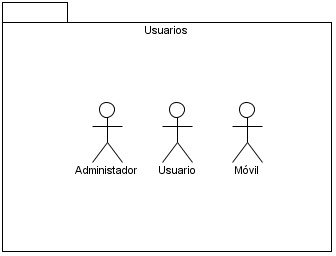
\includegraphics[width=0.7\textwidth]{ModeloComportamiento/imagenes/Actores.png}}
      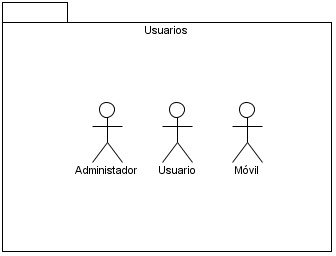
\includegraphics[width=0.6\textwidth]{ModeloComportamiento/imagenes/Actores.png}
      \caption{Perfiles identificados.}
      \label{fig:perfiles}
      \end{center}
    \end{figure}

\begin{actor}{Usuario}{Usuario}{Representa a cualquier persona que se registre u haga uso de la aplicación}
	\item[Actividades:]
	\item[Cantidad:] Uno por cada dispositivo móvil.
	
\end{actor}


\begin{actor}{Movil}{Móvil}{Representa el dispositivo móvil del usuario}
	\item[Actividades:]
	\item[Cantidad:] Uno por cada usuario.
	
\end{actor}

\begin{actor}{Administrador}{Administrador}{Representa al administrador de la aplicación}
	\item[Actividades:]
	\item[Cantidad:] Uno
	
\end{actor}